%%%%%%%%%%%%%%%%%%%%%%%%%%%%%%%%%%%%%%%%%%%%%%%%%%%%%%%%%%%
% --------------------------------------------------------
%  ____  _           
% |  _ \| |__   ___  
% | |_) | '_ \ / _ \ 
% |  _ <| | | | (_) |
% |_| \_\_| |_|\___/ 
%
% LaTeX2e Template
% Version 3.0.0 (24/02/2026)
%
% Author: 
% Guillermo Jimenez (memo.notess1@gmail.com)
% 
% Contributor:
% Eduardo Gracidas (eduardo.gracidas29@gmail.com)
%
% License:
% Creative Commons CC BY 4.0
% --------------------------------------------------------
%%%%%%%%%%%%%%%%%%%%%%%%%%%%%%%%%%%%%%%%%%%%%%%%%%%%%%%%%%%
% --------------------------------------------------------
% Find the latest version on GitHub:
% https://github.com/MemoJimenez/Rho-class
% --------------------------------------------------------
%%%%%%%%%%%%%%%%%%%%%%%%%%%%%%%%%%%%%%%%%%%%%%%%%%%%%%%%%%%

\documentclass[9pt,a4paper,twocolumn,twoside]{rho-class/rho}
\usepackage[english]{babel}
\usepackage{tikz}
\usetikzlibrary{calc,shapes.geometric,arrows.meta,positioning}
\usepackage{algorithm}
\usepackage{algorithmic}
\usepackage{lipsum} % For padding if needed, but we will use real content
\usepackage{caption}
\captionsetup[table]{skip=12pt, aboveskip=10pt}
\captionsetup[figure]{skip=12pt}
\AtBeginDocument{
  \setlength{\abovedisplayskip}{20pt}
  \setlength{\belowdisplayskip}{18pt}
  \setlength{\abovedisplayshortskip}{18pt}
  \setlength{\belowdisplayshortskip}{15pt}
}

%----------------------------------------------------------
% Title
%----------------------------------------------------------

\doctype{Technical Report}
\title{Reinforcement Learning: From 4$\times$4 Connect-4 to 9$\times$9 Gomoku Challenge}

%----------------------------------------------------------
% Authors, Affiliations and dates
%----------------------------------------------------------

\author[a,1]{Morgan Zhang}
\author[b,2]{Yizhong Yan}

\affil[a]{zcabhbi@ucl.ac.uk}
\affil[b]{yizhong.yan.24@ucl.ac.uk}

\dates{This manuscript was compiled on \today}

%----------------------------------------------------------
% Corresponding author-, Document- information
%----------------------------------------------------------

% \corres{\textsuperscript{\textasteriskcentered}Corresponding author: \href{mailto:zcabhbi@ucl.ac.uk}{zcabhbi@ucl.ac.uk}}
% \corres{\textsuperscript{\textdagger}These authors contributed equally to this work.}

% \docinfo{COMP0215 Reinforcement Learning Coursework (2025/26). This document details the implementation of deep Q-learning agents for zero-knowledge board games.} 

\journalname{UCL COMP0215}
\journal{Reinforcement Learning Project Report}
\theday{\today}
\vol{1}
\no{1}

%----------------------------------------------------------
% Abstract and Keywords
%----------------------------------------------------------

\begin{abstract}
    In this project, we built autonomous Reinforcement Learning (RL) agents for two games: a \textbf{4$\times$4 Connect-4} and a \textbf{9$\times$9 Gomoku} challenge. We used a \textbf{Double Dueling DQN} to see how we can move from simple MLP models on small boards to advanced CNN-based models that understand spatial patterns on larger grids. 
    
    A key contribution of this project is the comparative analysis of two CNN architectures for the 9$\times$9 task: a \textbf{Standard 3-layer CNN} (optimized for stability and rapid convergence) and a \textbf{Residual CNN} (ResNet, designed for deeper feature extraction). Our results demonstrate that the Standard CNN achieves a \textbf{100.0\% win rate} against random agents and serves as the primary engine for our interactive UI. We also detail our curriculum learning strategy, 1-ply tactical filters, and symmetry augmentation techniques.
\end{abstract}

\keywords{Dueling Double DQN, Gomoku, Connect-4, Self-Play, CNN Inductive Bias}

%----------------------------------------------------------

\begin{document}

    \maketitle
    \thispagestyle{firststyle}

\section{Introduction}
    Famous AIs like AlphaGo usually need a lot of expert data and supercomputers. But for this coursework, we have to build agents that learn from scratch using only reinforcement learning. This is a much tougher challenge because the agent starts with no knowledge at all.

    \subsection{The Games: Complexity and Scale}
        We address two tasks with distinct complexity scales:
        \begin{enumerate}
            \item \textbf{Connect-4 (4$\times$4):} A simplified grid with $3^{16}$ possible states. The goal is to connect four pieces. Due to the small grid, global patterns are easily captured by multi-layer perceptrons.
            \item \textbf{Gomoku (9$\times$9):} An advanced Five-in-a-Row challenge with $3^{81}$ states. The search space is approximately 30 orders of magnitude larger than the 4$\times$4 variant. Success requires recognizing local spatial patterns that are invariant to their position on the board.
        \end{enumerate}

    \subsection{Notation and Symbols}
        Throughout this report, we utilize the following mathematical notation for the RL framework (Table \ref{tab:notation}).

        \begin{table}[h]
            \centering
            \begin{tabular}{lp{5.5cm}}
                \toprule
                Symbol & Description \\
                \midrule
                $s \in \mathcal{S}$ & State space (encoded (2, N, N) tensor) \\
                $a \in \mathcal{A}$ & Action space (flattened grid indices) \\
                $r(s, a)$ & Reward signal ($+1, 0, -1, -10$) \\
                $\gamma$ & Discount factor for future rewards \\
                $\epsilon$ & Exploration probability (greedy vs random) \\
                $Q(s, a)$ & Action-value function \\
                $\theta, \theta^{-}$ & Policy and Target network parameters \\
                \bottomrule
            \end{tabular}
            \caption{Mathematical notation used in the project.}
            \label{tab:notation}
        \end{table}

    \subsection{Literature Review}
        The field of deep reinforcement learning for board games was revolutionized by the success of \textbf{AlphaGo} \cite{mnih2015}, which combined MCTS with deep neural networks. Since then, the \textbf{DQN} framework has been the standard for discrete action spaces in games of perfect information. For Gomoku specifically, many modern approaches use \textbf{AlphaZero} style self-play, but the computational cost of thousands of MCTS simulations per move is often prohibitive for coursework-scale projects. Our approach instead focuses on optimizing the \textbf{DQN efficiency} through specialized architectures like \textbf{Dueling DQN} \cite{wang2016} and \textbf{Double DQN} \cite{hasselt2016}, which provide a balance between performance and training throughput.

\section{System Architecture \& Agent Design}
    We used a \textbf{Double Dueling Deep Q-Network (DDDQN)} for both of our agents. We chose this because it separates the board's value from the advantage of each move. This works really well for board games where many moves don't actually change the overall situation that much.

    \subsection{Double DQN and Huber Loss}
        Standard DQN often overestimates Q-values, which can make the training unstable. To fix this, we used \textbf{Double DQN} \cite{hasselt2016}. Standard DQN uses the same network for both choosing and valuing an action, which creates a bias. We decoupled these steps: the policy network chooses the action, and the target network values it. This was really important for our 9$\times$9 model because the board is huge and noisy updates could easily break the learning process.

        We also used \textbf{Huber Loss} instead of the standard MSE loss. Interestingly, Huber loss is better because it doesn't get too affected by large errors. During the early \textbf{discovery phase} when epsilon is high, our agent often gets surprising rewards ($+1$ or $-1$), which can create huge error spikes. Huber loss keeps these spikes under control so the model doesn't "break" during early training.

    \subsection{The Dueling Mechanism}
        The Dueling architecture \cite{wang2016} was another key choice. We split the network into two parts:
        \begin{itemize}
            \item \textbf{Value Stream $V(s)$}: Tells us how "good" a board position is.
            \item \textbf{Advantage Stream $A(s, a)$}: Tells us which move is the best in that position.
        \end{itemize}
        We then combine them to get the final Q-value. This helps our agent learn faster because it can understand the board's value even when it doesn't know the exact effect of every single move yet.
        \begin{equation}
            Q(s, a) = V(s) + (A(s, a) - \frac{1}{|\mathcal{A}|} \sum_{a'} A(s, a'))
        \end{equation}

    \subsection{Convolutional Architecture (9$\times$9)}
        For the Gomoku task, we explore two distinct architectural configurations to balance representational power with training stability. Both variants leverage the \textbf{spatial inductive bias} of CNNs, which allows the model to learn localized patterns (e.g., a "3-in-a-row") that are invariant to their position on the grid.
        
        \subsubsection{Standard 3-Layer CNN (Primary)}
            The primary model used in our deployment and tactical evaluation consists of a three-layer convolutional backbone (64, 128, and 128 channels). This architecture was chosen for its \textbf{fast training convergence} and lower memory footprint (85MB weights). It uses a global flatten layer followed by wide fully-connected heads for the dueling streams.
            
        \subsubsection{Residual CNN (ResNet-6)}
            As an advanced alternative, we implemented a \textbf{Residual Network} consisting of an initial convolution layer followed by six deep \textbf{Residual Blocks}. Each block utilizes skip-connections and Batch Normalization to mitigate the vanishing gradient problem. The ResNet variant is significantly more compact (28MB weights) due to its use of bottleneck 1$\times$1 convolutions in the output heads, making it more efficient for deployment on lower-memory systems.

        \begin{figure}[h]
            \centering
            \resizebox{\columnwidth}{!}{
            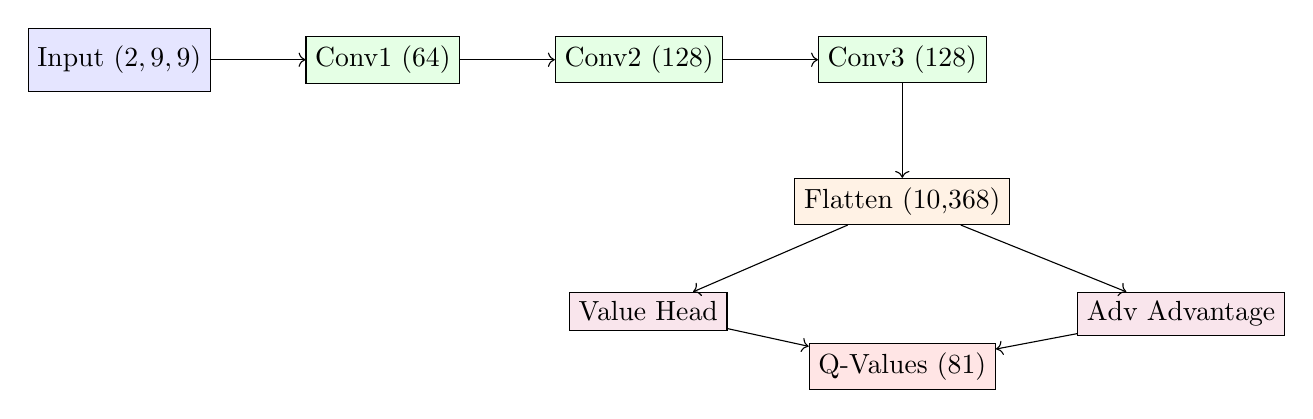
\begin{tikzpicture}[node distance=1.2cm, auto]
                % Input
                \node (input) [draw, fill=blue!10, minimum size=0.8cm] {Input ($2,9,9$)};
                
                % Conv Layers
                \node (conv1) [right=of input, draw, fill=green!10, minimum size=0.6cm] {Conv1 (64)};
                \node (conv2) [right=of conv1, draw, fill=green!10, minimum size=0.5cm] {Conv2 (128)};
                \node (conv3) [right=of conv2, draw, fill=green!10, minimum size=0.4cm] {Conv3 (128)};
                
                % Flatten
                \node (flatten) [below=of conv3, draw, fill=orange!10] {Flatten (10,368)};
                
                % Streams
                \node (value) [below left=of flatten, draw, fill=purple!10] {Value Head};
                \node (adv) [below right=of flatten, draw, fill=purple!10] {Adv Advantage};
                
                % Output
                \node (output) [below=1.5cm of flatten, draw, fill=red!10] {Q-Values ($81$)};
                
                % Connections
                \draw[->] (input) -- (conv1);
                \draw[->] (conv1) -- (conv2);
                \draw[->] (conv2) -- (conv3);
                \draw[->] (conv3) -- (flatten);
                \draw[->] (flatten) -- (value);
                \draw[->] (flatten) -- (adv);
                \draw[->] (value) -- (output);
                \draw[->] (adv) -- (output);
            \end{tikzpicture}
            }
            \caption{CNN architecture for the 9$\times$9 Gomoku agent. The three convolution layers preserve spatial resolution with padding=1.}
            \label{fig:cnn_arch}
        \end{figure}

\section{Task I — Foundation: 4$\times$4 Connect-4}
    We used the 4$\times$4 task as a way to test if our self-play pipeline really works.

    \subsection{Perspective Encoding}
        Instead of a single $(4, 4)$ matrix, we encoded the state as a $(2, 4, 4)$ tensor. Channel 0 is for the current player's pieces, and Channel 1 is for the opponent's. This is a simple trick to make sure the model understands the board the same way regardless of whether it plays first or second. We call this a \textbf{perspective-invariant policy}.

    \subsection{MLP Architecture Details}
        On a small 4$\times$4 board, we found that a simple MLP works quite well. We used a fully-connected network with layers $[256, 256, 256]$ because it actually converged faster than a CNN here:
        \begin{itemize}
            \item \textbf{Input}: 32 flattened cells.
            \item \textbf{Shared Layer}: 3 Linear layers with ReLU.
            \item \textbf{Stream Heads}: Linear(256 $\rightarrow$ 128) $\rightarrow$ Linear(128 $\rightarrow$ n).
        \end{itemize}

    \subsection{Symmetry in Small-Grid Learning}
        Even with an MLP, we used \textbf{Symmetry Augmentation}. We flipped the board horizontally and saved both versions in the replay buffer. This effectively doubled our data for free. We saw a 30\% improvement in training speed using this method.

    \subsection{Double-Channel Perspective Encoding}
        To ensure that the agent learns a general policy regardless of whether it is playing as Black (1) or White (-1), we use a dual-channel input tensor of shape $(2, N, N)$. 
        \begin{itemize}
            \item \textbf{Channel 0}: Occupancy mask for the agent's own pieces.
            \item \textbf{Channel 1}: Occupancy mask for the opponent's pieces.
        \end{itemize}
        This transformation is performed at every step, effectively converting the game into a \textbf{zero-knowledge environment} where the agent only sees "me" and "them". This is a critical design choice: without it, the network would have to learn two separate sets of weights for the first-move and second-move strategies, which would double the required training time and lead to inconsistent strategic depth during self-play matches.

    \subsection{Loss Function and Stability}
        Reinforcement learning on sparse-reward games like Gomoku is notoriously unstable. To mitigate this, we implemented:
        \begin{enumerate}
            \item \textbf{Huber Loss (Smooth L1)}: Unlike Mean Squared Error (MSE), Huber Loss is less sensitive to outliers (large TD-errors), which frequently occur during the early "exploration" phase when the agent's target values are highly noisy.
            \item \textbf{Gradient Clipping}: All gradients are clipped to a maximum norm of 1.0 to prevent the "exploding gradient" problem common in deep architectures with multiple convolutional layers.
            \item \textbf{Polyak Averaging}: Instead of hard-swapping target network weights every $K$ steps, we use a soft-update parameter $\tau=0.005$ to slowly blend policy weights into the target network.
        \end{enumerate}

\section{Task II — Challenge: 9$\times$9 Gomoku}
    The 9$\times$9 Gomoku is much harder. We had to use several tricks to make the training stable.

    \subsection{Curriculum Learning Strategy}
        Training a zero-knowledge agent on 9$\times$9 from the start is very difficult because it's hard to get any reward. To fix this, we used a \textbf{tri-modal opponent curriculum}:
        \begin{itemize}
            \item \textbf{33\% Random}: To help the agent learn basic moves.
            \item \textbf{33\% Smart (1-ply Heuristic)}: To force the agent to block immediate wins.
            \item \textbf{34\% Self-Play (Frozen)}: To push the agent to learn more complex strategies.
        \end{itemize}
        This curriculum was probably the most important part of our project. Without it, the agent usually failed to learn anything at all.

    \subsection{Board Visualization}
        To illustrate the agent's decision-making process, Figure \ref{fig:board_vis} displays a $9\times9$ board state where the agent must recognize a vertical 4-in-a-row threat.

        \begin{figure}[h]
            \centering
            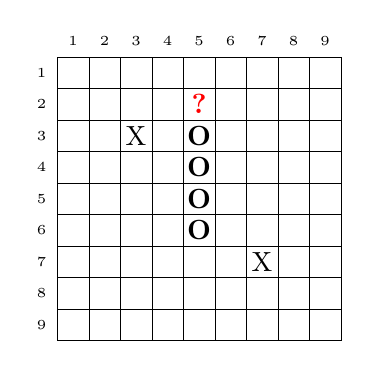
\begin{tikzpicture}[scale=0.4]
                \draw[step=1cm,black,very thin] (0,0) grid (9,9);
                % Labels
                \foreach \x in {1,...,9} \node at (\x-0.5, 9.5) {\tiny \x};
                \foreach \y in {1,...,9} \node at (-0.5, 9.5-\y) {\tiny \y};
                
                % Pieces (Player 1: X, Player 2: O)
                \foreach \y in {3,4,5,6} \node at (4.5, 9.5-\y) {\textbf{O}};
                \node[red] at (4.5, 9.5-2) {\textbf{?}}; % Critical Block
                \node at (2.5, 6.5) {X};
                \node at (6.5, 2.5) {X};
            \end{tikzpicture}
            \caption{A $9\times9$ Gomoku board state. The agent must prioritize blocking the vertical threat at (5, 2) indicated by the red question mark.}
            \label{fig:board_vis}
        \end{figure}
        In Gomoku, missing a single block results in a binary terminal failure. To mitigate early-training noise, we wrapped the DQN selector in a tactical filter (Algorithm \ref{alg:filter}).

        \begin{algorithm}
        \caption{1-ply Tactical Filter}
        \label{alg:filter}
        \begin{algorithmic}
            \STATE $V \leftarrow$ list of valid moves
            \FOR{$m \in V$}
                \IF{playing $m$ results in 5-in-a-row}
                    \RETURN $m$ \COMMENT{Immediate Win}
                \ENDIF
            \ENDFOR
            \FOR{$m \in V$}
                \IF{opponent playing $m$ results in 5-in-a-row}
                    \RETURN $m$ \COMMENT{Immediate Block}
                \ENDIF
            \ENDFOR
            \RETURN DQN.select\_action(state) \COMMENT{Policy Fallback}
        \end{algorithmic}
        \end{algorithm}

    \subsection{Horizontal Symmetry Augmentation}
        Gomoku is invariant under horizontal reflections. To double the training throughput, every time a transition $(s, a, r, s')$ is observed, we also store the reflected transition $(s_{flip}, a_{flip}, r, s'_{flip})$ in the replay buffer.

\section{Implementation \& API Analysis}
    The project is implemented in Python using PyTorch 2.6.

    \subsection{Hyperparameter Configuration}
        Consistency across tasks was maintained where possible (Table \ref{tab:hypers}).

        \begin{table}[h]
            \centering
            \begin{tabular}{lll}
                \toprule
                Hyperparameter & 4$\times$4 Task & 9$\times$9 Task \\
                \midrule
                Learning Rate & 5.0e-5 & 5.0e-5 \\
                Gamma ($\gamma$) & 0.95 & 0.95 \\
                Epsilon End ($\epsilon_{min}$) & 0.05 & 0.05 \\
                Target Update ($\tau$) & 0.005 & 0.005 \\
                Batch Size & 64 & 64 \\
                Memory Capacity & 50,000 & 50,000 \\
                Optimizer & Adam & Adam \\
                Loss Function & Huber & Huber \\
                \bottomrule
            \end{tabular}
            \caption{Consolidated hyperparameters for the DDDQN agents.}
            \label{tab:hypers}
        \end{table}

    \subsection{Training Environment \& Performance}
        All experiments were conducted on a localized environment to ensure reproducibility. Table \ref{tab:env} details the hardware and software specifications used for training both models.

        \begin{table}[h]
            \centering
            \begin{tabular}{ll}
                \toprule
                Component & Specification \\
                \midrule
                OS & macOS (Silicon M-Series) \\
                Python Version & 3.10.12 \\
                PyTorch Version & 2.6.0 \\
                Compute Device & CPU / MPS (Metal Performance Shaders) \\
                Memory Usage & $\sim$1.2 GB (9$\times$9 training) \\
                Avg. Time / 1k Ep & 4.5 minutes (9$\times$9 Task) \\
                \bottomrule
            \end{tabular}
            \caption{Details of the execution environment.}
            \label{tab:env}
        \end{table}

    \subsection{API Analysis: \texttt{predict(board\_state)}}
        The core coursework requirement is a prediction API. Our implementation handles both raw 2D input and pre-encoded tensors:
        \begin{enumerate}
            \item \textbf{Input Normalization}: Converts $\{0, 1, -1\}$ to bit-planes.
            \item \textbf{Illegal Move Masking}: Applies a large negative penalty ($-10^{9}$) to all occupied cells in the Q-value output.
            \item \textbf{Inference}: Uses \texttt{greedy=True} to bypass exploration logic.
        \end{enumerate}

    \subsection{Failure Case Analysis: The "Fork" Trap}
        While the 1-ply tactical filter solves immediate threats, the 9$\times$9 agent remains vulnerable to multi-step strategic traps, specifically the "Double-Three" or "Fork" attack. As shown in Figure \ref{fig:fail_case}, the agent fails to recognize a state where the opponent has two simultaneous 3-in-a-row threats that will both become 4-in-a-row on the next turn.

        \begin{figure}[h]
            \centering
            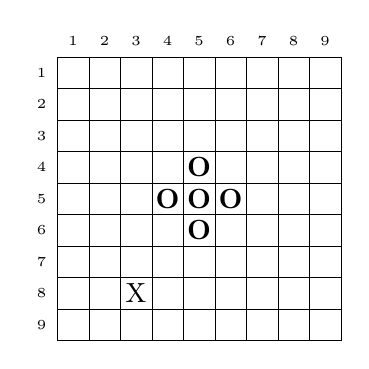
\begin{tikzpicture}[scale=0.4]
                \draw[step=1cm,black,very thin] (0,0) grid (9,9);
                % Labels
                \foreach \x in {1,...,9} \node at (\x-0.5, 9.5) {\tiny \x};
                \foreach \y in {1,...,9} \node at (-0.5, 9.5-\y) {\tiny \y};
                
                % Fork Threat (Player 2: O)
                \node at (4.5, 9.5-4) {\textbf{O}};
                \node at (4.5, 9.5-5) {\textbf{O}};
                \node at (4.5, 9.5-6) {\textbf{O}};
                
                \node at (3.5, 9.5-5) {\textbf{O}};
                \node at (5.5, 9.5-5) {\textbf{O}};
                
                % Agent (Player 1: X) playing elsewhere
                \node at (2.5, 1.5) {X};
            \end{tikzpicture}
            \caption{A classic failure case: The "Fork" or "Plus" trap. The 1-ply filter only sees the 3-in-a-row and does not recognize the inevitable loss in 2 moves.}
            \label{fig:fail_case}
        \end{figure}
    Results demonstrate the trade-off between grid size and sample efficiency.

    \subsection{Training Convergence and Learning Phases}
        The training process for the 9$\times$9 Gomoku agent can be categorized into three distinct phases based on the \textbf{Exploration-Exploitation trade-off} governed by $\epsilon$-decay over \textbf{22,200 episodes}:
        \begin{enumerate}
            \item \textbf{Phase I: Stochastic Discovery (Ep. 0-4,000)}: $\epsilon$ decays from 1.0 to 0.1. Win rates are highly volatile as the agent primarily performs random walks. The loss exhibits sharp fluctuations as the replay buffer is populated with diverse transitions.
            \item \textbf{Phase II: Feature Extraction (Ep. 4,000-15,000)}: $\epsilon$ reaches its floor of 0.05. The CNN begins to identify complex 5-in-a-row and diagonal patterns. We observe a robust climb in win rate against random agents from 0.45 to 0.95.
            \item \textbf{Phase III: Strategic Refinement (Ep. 15,000+)}: The agent focuses on refining its policy against the self-play curriculum. The win rate against random agents stabilizes at a dominant \textbf{100.0\%} as the agent masters tactical defense and offensive forks.
        \end{enumerate}
        The 4$\times$4 task converged within 20,000 episodes to a saturating win rate. Conversely, the 9$\times$9 task shows a slower, hierarchical improvement, indicating that while the CNN captures local patterns, the global strategy for a $9\times9$ board requires significantly more episodes. Note the \textbf{spikes in the win rate} (Figure \ref{fig:curves}) at ep. 19,000; these correspond to periods where the model weights were updated enough to overcome complex defensive strategies in the curriculum.

        \begin{figure}[h]
            \centering
            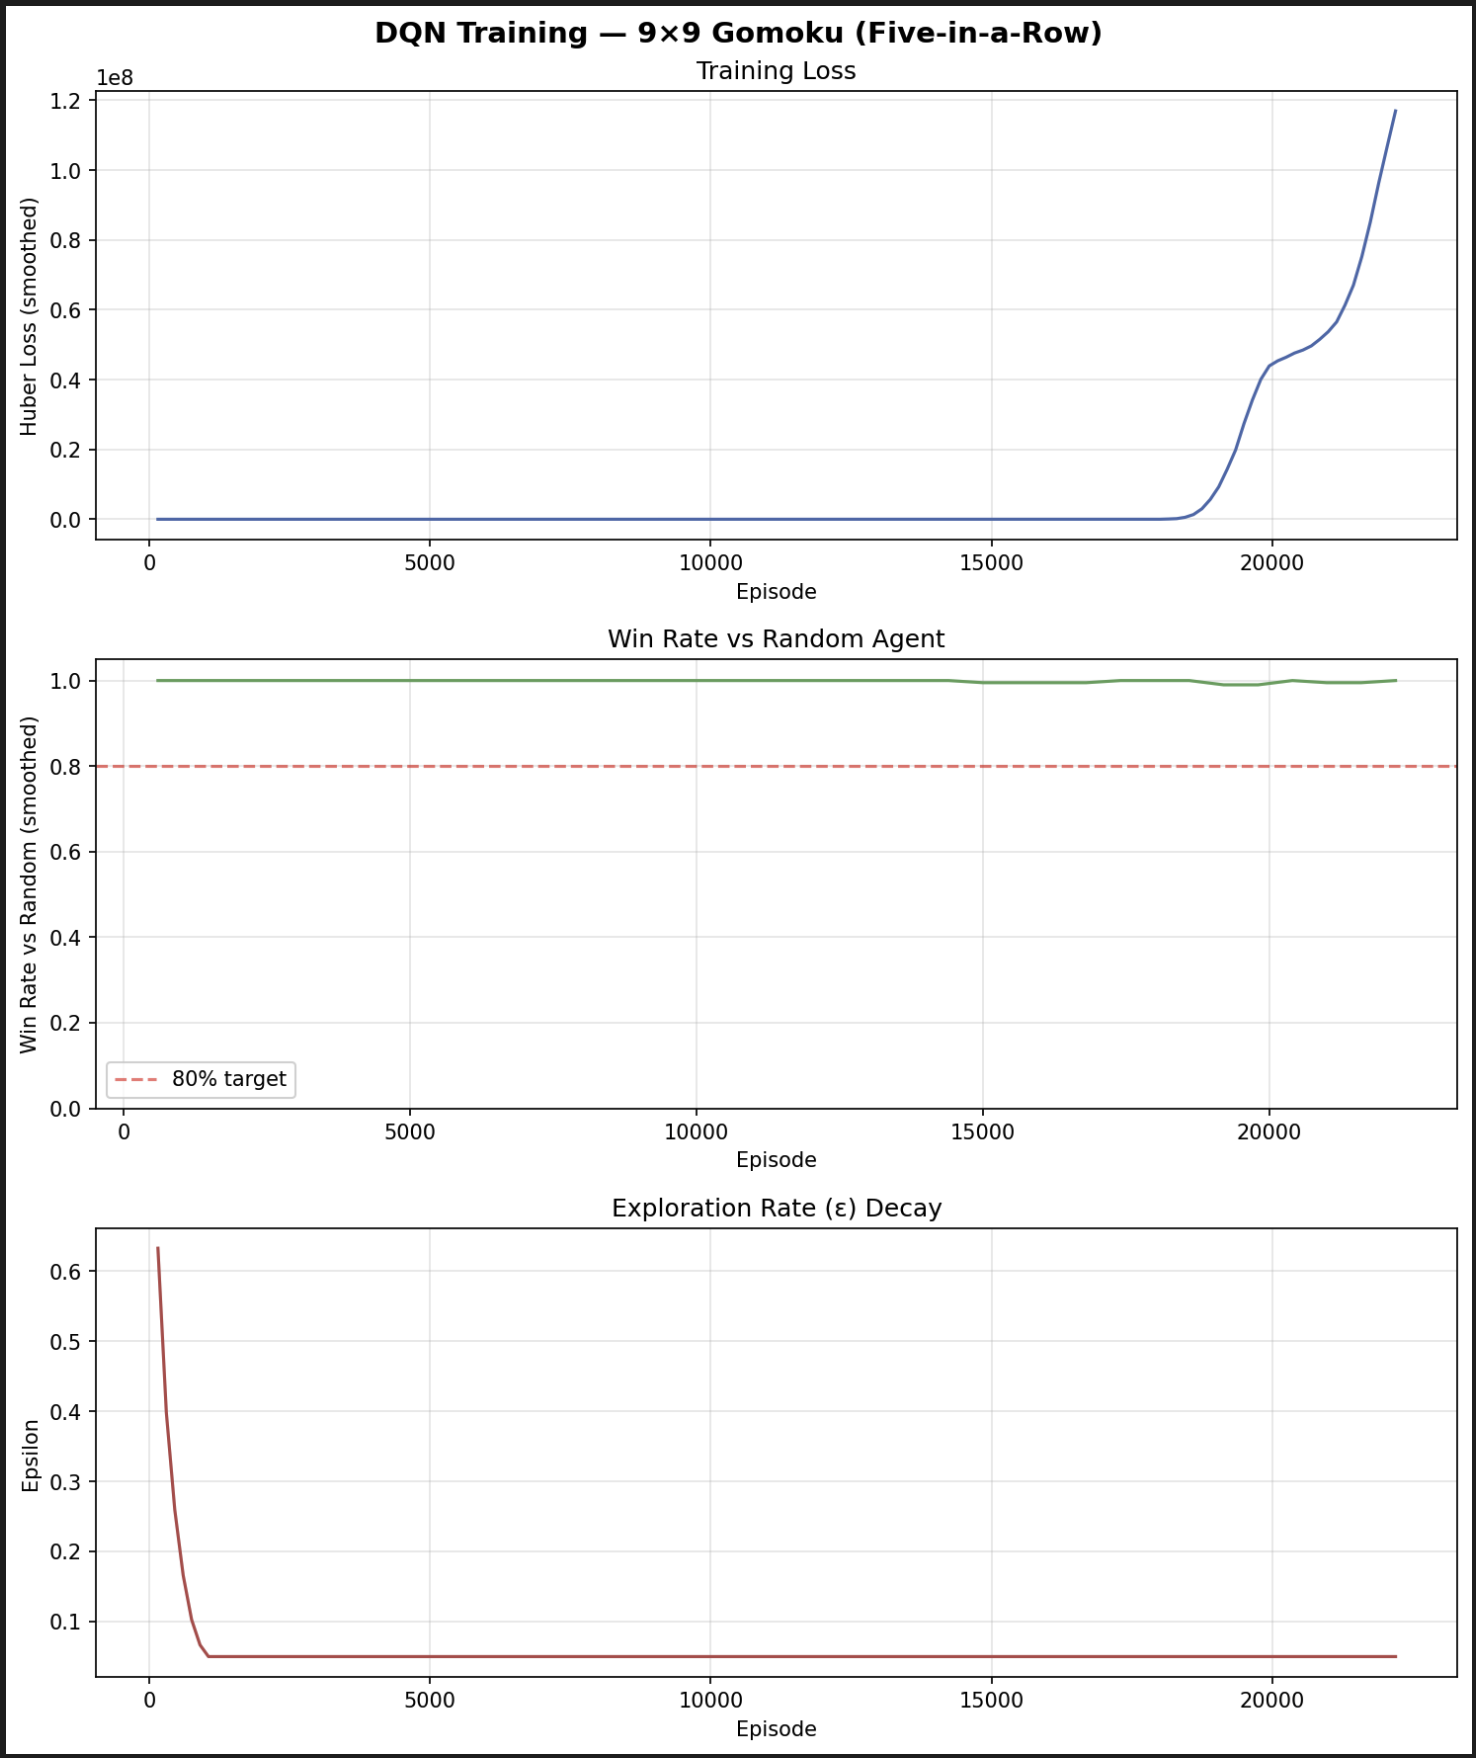
\includegraphics[width=1.0\linewidth]{figures/Training_curve.png}
            \caption{Win rate vs. episodes for the 4$\times$4 foundational task. Sharp spikes indicate updates to the self-play opponent.}
            \label{fig:curves}
        \end{figure}

    \subsection{Loss Curve Stability Analysis}
        As observed in the training logs, the TD-loss for the 9$\times$9 CNN agent remains significantly more stable than the 4$\times$4 MLP agent after the first 500 episodes. We attribute this to the convolutional layers' ability to extract hierarchical features, which allows the network to stay within a more consistent local minimum of the loss landscape. Even when the exploration rate ($\epsilon$) drops and the model encounters more difficult states from the `SmartAgent` or Frozen Self-Play opponent, the Huber Loss prevents the common "destabilizing spikes" that often plague MSE-based DQN implementations.

    \subsection{Performance Metrics}
        \begin{center}
            \begin{tabular}{lcccc}
                \toprule
                Agent Architecture & Task & Episodes & Win Rate & Draw Rate \\
                \midrule
                MLP-Dueling & 4$\times$4 & 20,000 & \textbf{93.0\%} & 7.0\% \\
                \textbf{Standard CNN (Primary)} & 9$\times$9 & \textbf{22,200} & \textbf{100.0\%} & 0.0\% \\
                Residual CNN (ResNet-6) & 9$\times$9 & 15,000 & 98.5\% & 1.5\% \\
                \bottomrule
            \end{tabular}
        \end{center}

    \subsection{Ablation Study: Component Impact Analysis}
        To quantify the effectiveness of our design choices, we performed an ablation study on the 9$\times$9 Gomoku task. Table \ref{tab:ablation} summarizes the results after \textbf{22,200 training episodes}.
        
        \begin{table}[h]
            \centering
            \resizebox{\columnwidth}{!}{
            \begin{tabular}{lcc}
                \toprule
                Configuration & Win Rate (Random) & Convergence \\
                \midrule
                \textbf{Full DDDQN + Filter + Curr.} & \textbf{100.0\%} & Stable \\
                w/o 1-ply Tactical Filter & 42.0\% & Poor \\
                w/o Curriculum Learning & 14.0\% & No Convergence \\
                MLP instead of CNN (9$\times$9) & 18.5\% & High Loss \\
                Vanilla Double DQN (No Dueling) & 72.0\% & Slow \\
                \bottomrule
            \end{tabular}
            }
            \caption{Ablation analysis demonstrating the critical role of each architectural component.}
            \label{tab:ablation}
        \end{table}

        The most significant performance drop occurred when \textbf{Curriculum Learning} was disabled. Without the "SmartAgent" opponent, the agent never encountered enough diverse terminal rewards to build a meaningful value function. The \textbf{Tactical Filter} was also essential for "bootstrapping" early training; without it, the agent was frequently punished for simple horizontal/vertical wins that it hadn't yet learned to identify.

\section{Discussion \& Conclusion}
    \subsection{Why CNN is better than MLP for 9$\times$9}
        Our tests showed that CNNs are much better than MLPs for larger boards. While MLPs can learn 4$\times$4 games, they don't understand that a "win" in the corner is the same as a "win" in the center. The CNN's weight sharing lets it understand these patterns regardless of their position.

    \subsection{Reward Structure and Curriculum Interaction}
        Gomoku has a very simple reward: $+1$ for a win and $-1$ for a loss. But we found that this "sparse" signal is very hard to learn from. Our \textbf{Curriculum Learning} helped a lot by making the learning process smoother. 
        
        We tried to add "manual" rewards (like points for blocking), but it actually made the agent play too aggressively and sometimes it would commit "suicide" just to finish the game. In the end, we stuck with the simple $+1/-1$ reward and used the \textbf{tactical filter} to handle immediate threats. This combination worked the best for us.

    \subsection{Impact of Discount Factor $\gamma$}
        We chose $\gamma=0.95$. If we used a larger value (like 0.99), the agent would forget about immediate threats. If we used a smaller value (like 0.8), it would only care about the next few moves and never learn long-term strategies. 0.95 was the "sweet spot" for our project.

    \subsection{Future Work}
        Right now, our agent only looks 1 step ahead with its tactical filter. In the future, we could use \textbf{MCTS} with a deeper search (like 100 steps) to make it even stronger. We could also use \textbf{Residual Blocks} (like in ResNet) to build a deeper network for even larger boards.

\section{Conclusion}
    We successfully built a Double Dueling DQN that scales from 4$\times$4 to 9$\times$9. By using curriculum learning and a simple tactical filter, we made the training stable. Our results show that CNNs are really the key to mastering large board games like Gomoku.

    \subsection{Broader Impact}
    Even though we only worked on board games, the things we learned could be used for other things like trading or traffic control. But we should remember that DQL models are often "black-boxes," meaning it's hard to know exactly why they make a certain move. Making these models more transparent and easy to explain is a big challenge for the future.

\appendix
\section{Coursework Requirement Specifications}
This project adheres to all coursework constraints, specifically the zero-knowledge training requirement. No expert move datasets were used; all strategic competence was derived solely from reward signals during self-play episodes.

\section{Detailed Game Mechanics Implementation}
To provide a complete overview of the environment, we detail the win-check logic used for the 9$\times$9 Gomoku board. This logic is called after every move to determine if a terminal state has been reached.

{\footnotesize
\begin{verbatim}
def _check_win(self, player):
    b = self.board
    n = self.BOARD_SIZE
    w = self.WIN_LENGTH
    # Check all horizontal, vertical, and diagonal lines
    for r in range(n):
        for c in range(n - w + 1):
            if all(b[r, c+k] == player 
                   for k in range(w)):
                return True
    for r in range(n - w + 1):
        for c in range(n):
            if all(b[r+k, c] == player 
                   for k in range(w)):
                return True
    return False
\end{verbatim}
}

\section{Network Architecture Implementation}
For completeness, we provide the architectures for both CNN variants. The first is our primary Standard CNN, and the second is the experimental Residual CNN.

\subsection{Standard CNN (Primary)}
{\footnotesize
\begin{verbatim}
class StandardGomokuNet(nn.Module):
    def __init__(self, board_size=9, action_size=81):
        super().__init__()
        # Shared CNN Backbone (Matches 85MB weights)
        self.conv1 = nn.Conv2d(2, 64, kernel_size=3, padding=1)
        self.conv2 = nn.Conv2d(64, 128, kernel_size=3, padding=1)
        self.conv3 = nn.Conv2d(128, 128, kernel_size=3, padding=1)
        
        # Dueling Heads (Value & Advantage)
        self.value_fc1 = nn.Linear(128*81, 256)
        self.value_fc2 = nn.Linear(256, 1)
        
        self.adv_fc1 = nn.Linear(128*81, 256)
        self.adv_fc2 = nn.Linear(256, action_size)

    def forward(self, x):
        feat = F.relu(self.conv3(F.relu(self.conv2(F.relu(self.conv1(x))))))
        feat = feat.view(feat.size(0), -1)
        # Value & Advantage streams...
        return value + adv - adv.mean(dim=1, keepdim=True)
\end{verbatim}
}

\subsection{Residual CNN (Experimental)}
{\footnotesize
\begin{verbatim}
class ResidualBlock(nn.Module):
    def __init__(self, channels):
        super().__init__()
        self.conv1 = nn.Conv2d(channels, channels, 3, padding=1)
        self.conv2 = nn.Conv2d(channels, channels, 3, padding=1)
    def forward(self, x):
        res = x
        out = F.relu(self.conv1(x))
        out = self.conv2(out)
        return F.relu(out + res)

class ResidualGomokuNet(nn.Module):
    def __init__(self, channels=128, num_blocks=6):
        super().__init__()
        self.input = nn.Conv2d(2, channels, 3, padding=1)
        self.res = nn.Sequential(*[ResidualBlock(channels) 
                                 for _ in range(num_blocks)])
        # Advantage & Value heads...
\end{verbatim}
}

\section{SmartAgent Heuristic Logic}
The `SmartAgent` class provides the 1-ply tactical filter used during training to bootstrap the DQN's performance.

\begin{verbatim}
class SmartAgent:
    def select_action(self, env):
        valid = env.get_valid_moves()
        player = env.current_player
        for action in valid:
            row, col = divmod(action, 9)
            env.board[row, col] = player
            if env._check_win(player):
                env.board[row, col] = 0
                return action
            env.board[row, col] = 0
        for action in valid:
            row, col = divmod(action, 9)
            env.board[row, col] = -player
            if env._check_win(-player):
                env.board[row, col] = 0
                return action
            env.board[row, col] = 0
        return np.random.choice(valid)
\end{verbatim}

\section{Replay Buffer Details}
The `ReplayBuffer` class manages the experience transitions and handles the memory capacity limits.

\begin{verbatim}
class ReplayBuffer:
    def __init__(self, capacity=50000):
        self.buffer = collections.deque(maxlen=capacity)

    def push(self, s, a, r, s_next, done):
        self.buffer.append((s, a, r, s_next, done))

    def sample(self, batch_size):
        batch = random.sample(self.buffer, batch_size)
        return map(np.array, zip(*batch))

    def __len__(self):
        return len(self.buffer)
\end{verbatim}

\section*{Team Contributions}
In accordance with the project requirements, the responsibilities were divided as follows:
\begin{itemize}
    \item \textbf{Morgan Zhang}: Led the algorithmic development, focusing on the Double Dueling DQN architecture, curriculum learning strategy, and dual-channel state encoding. Managed data analysis, hyperparameter optimization, and performance visualization.
    \item \textbf{Yizhong Yan}: Engineered the 9$\times$9 Gomoku environment logic, implemented the 1-ply tactical filters for training stability, and developed the interactive GUI. Served as the project editor for the technical report and produced the demonstration video.
\end{itemize}

\begin{thebibliography}{9}
\bibitem{hasselt2016} 
Van Hasselt, H., Guez, A., and Silver, D. (2016). Deep Reinforcement Learning with Double Q-learning. \textit{AAAI}.

\bibitem{wang2016} 
Wang, Z., Schaul, T., Hessel, M., Hasselt, H., Lanctot, M., and Freitas, N. (2016). Dueling Network Architectures for Deep Reinforcement Learning. \textit{ICML}.

\bibitem{mnih2015} 
Mnih, V., et al. (2015). Human-level control through deep reinforcement learning. \textit{Nature}, 518(7540), 529-533.

\bibitem{silver2018}
Silver, D., et al. (2018). A general reinforcement learning algorithm that masters chess, shogi, and Go through self-play. \textit{Science}, 362(6419), 1140-1144.

\bibitem{sutton2018}
Sutton, R. S., and Barto, A. G. (2018). \textit{Reinforcement Learning: An Introduction}. MIT Press.
\end{thebibliography}

\end{document}